\documentclass{article}
\usepackage[en]{ukon-infie}
\usepackage[utf8]{inputenc}
\usepackage{algorithm2e}
\usepackage{amsmath}
\usepackage{graphicx}
\usepackage{hyperref}
% kann de oder en sein
% kann bubble break, topexercise sein

\Names{Jonas Probst, Simon Giebenhain}
\Lecture[AnaVis]{Analyse und Visualisierung von Informationen}
\Term{WS 2017/18}

\begin{document}
    \begin{ukon-infie}[24.01.18]{10}

        \begin{exercise}[p=6]{Gestalt Laws}  
        \question{}
        {
      	\begin{enumerate}
      	\item \textbf{Proximity}: In the left diagramm the points are percieved as clusters.
      	\item Similarity
      	\item \textbf{Connectedness}: In the right diagramm the points are not  percieved as clusters anymore, but as time-series data.
      	\item Continuity
      	\item \textbf{Figure and Ground}: The axes and points are clearly identified to be in the foreground.
      	\item Symmetry
      	\end{enumerate}
      	}
      	
      	\question{}
      	{
      		On the left hand side, the proximity of the points has the biggest influence on our perception. Therefore, it is easy to percieve them in clusters and ignore the time axis, instead of regarding them as time-series data.\\
      		On the right hand side the line connecting the data points underlines their chronological relation, which helps to see the diagramm as intended.
      	}
		\end{exercise}
		
		
		\begin{exercise}[p=2]{Pre-attentive Perception}
		\question{}
		{
		Pre-attentive perception describes a kind of perception, in which the user percieves the object of interest immediately, without spending any concious thoughts about it.
		}
		\question{}
		{
			One example would be locating your current postion on a map, e.g. in a navigation system, as it can be seen on the screenshot below. In such a case it is extremely helpful to have a clearly visibile marker enabeling preattentive perception, because often the map is loaded with details, making it hard to make out your location, without this obvious marker. Furthermore the view of the user continously jumps from his/her current location to his/her destination, when planning a route.\\
			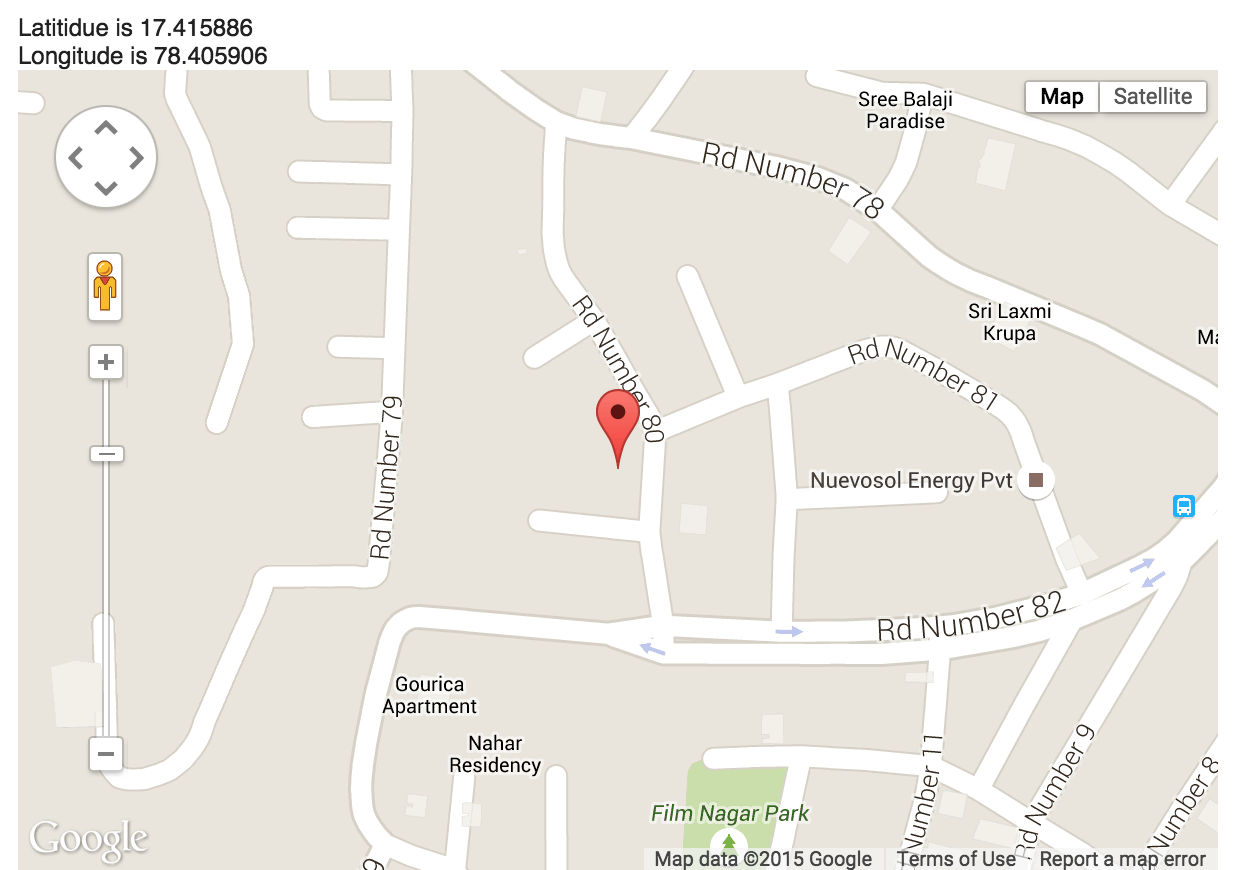
\includegraphics[scale=0.4]{preattentive_perception.png}
		}
		\end{exercise}
		
		\begin{exercise}[p=4]{Pixel-oriented Visualization}
		
		\end{exercise}
		
		
\end{ukon-infie}
\end{document}
